%%%%%%%%%%%%%%%%%%%%%%%%%%%%%%%%%%%%%%%%%
% Beamer Presentation
% LaTeX Template
% Version 1.0 (10/11/12)
%
% This template has been downloaded from:
% http://www.LaTeXTemplates.com
%
% License:
% CC BY-NC-SA 3.0 (http://creativecommons.org/licenses/by-nc-sa/3.0/)
%
%%%%%%%%%%%%%%%%%%%%%%%%%%%%%%%%%%%%%%%%%

%----------------------------------------------------------------------------------------
%	PACKAGES AND THEMES
%----------------------------------------------------------------------------------------

\documentclass{beamer}

\mode<presentation> {

\usetheme{Madrid}
\usecolortheme{dolphin}
%\setbeamertemplate{footline} % To remove the footer line in all slides uncomment this line
%\setbeamertemplate{footline}[page number] % To replace the footer line in all slides with a simple slide count uncomment this line

%\setbeamertemplate{navigation symbols}{} % To remove the navigation symbols from the bottom of all slides uncomment this line
}

\usepackage{graphicx} % Allows including images
\usepackage{ragged2e} % Jusitfy
\usepackage{booktabs} % Allows the use of \toprule, \midrule and \bottomrule in tables
\usepackage{lmodern}
\usepackage{amsfonts}
\usepackage{amsmath}
\usepackage{mathtools}
\usepackage{multicol}
\usepackage{listings} % C++ code
\lstset{language=C++,
                basicstyle=\footnotesize\ttfamily,
                keywordstyle=\footnotesize\color{blue}\ttfamily,
}
\addtobeamertemplate{block begin}{}{\justifying} %Justify
%----------------------------------------------------------------------------------------
%	TITLE PAGE
%----------------------------------------------------------------------------------------

\title[AVR Set Instructions Analysis]{AVR Set Instructions Analysis} % The short title appears at the bottom of every slide, the full title is only on the title page

\author{Ulises M\'endez Mart\'{i}nez} % Your name
\institute[UAG] % Your institution as it will appear on the bottom of every slide, may be shorthand to save space
{
Universidad Aut\'onoma de Guadalajara  \\ % Your institution for the title page
\medskip
\textit{ulisesmdzmtz@gmail.com} % Your email address
}
\date{\today} % Date, can be changed to a custom date

\begin{document}

\begin{frame}
\titlepage % Print the title page as the first slide
\end{frame}


%--------------------------------------------------------
%	PRESENTATION SLIDES
%--------------------------------------------------------

%--------------------------------------------------------
%--------------------------------------------------------
\section{Instruction Summary} 
\subsection{Blocks of 256 instructions}
\begin{frame}
\frametitle{Summary Table I}
\small
\begin{center}
    \begin{tabular}{| l | l | l | l | l | l | l | l | l |}
    \hline
    - & x0zz & x1zz & x2zz & x3zz & x4zz & x5zz & x6zz & x7zz \\    \hline
    0xzz & [R] nop & movw & muls & fmul & cpc & cpc & cpc  & cpc \\ \hline
    1xzz & cpse & cpse & cpse & cpse & cp & cp & cp & cp \\ \hline
    2xzz & and & and & and & and & eor & eor & eor & eor \\ \hline
    3xzz & cpi & cpi & cpi & cpi & cpi & cpi & cpi & cpi \\ \hline
    4xzz & sbci & sbci & sbci & sbci & sbci & sbci & sbci & sbci \\ \hline
    5xzz & subi & subi & subi & subi & subi & subi & subi & subi \\ \hline
    6xzz & ori & ori & ori & ori & ori & ori & ori & ori \\ \hline
    7xzz & andi & andi & andi & andi & andi & andi & andi & andi \\ \hline
    8xzz & ld & ldd & st & std & ldd & ldd & std & std \\ \hline
    9xzz & MISC & MISC & [R] push &  st sts & MISC & MISC & adiw & sbiw \\ \hline
    Axzz & ldd & ldd & std & std & ldd & ldd & std  & std \\ \hline
    Bxzz & in & in & in & in & in & in & in & in \\ \hline
    Cxzz & rjmp & rjmp & rjmp & rjmp & rjmp & rjmp & rjmp & rjmp \\ \hline
    Dxzz & rcall & rcall & rcall & rcall & rcall & rcall & rcall & rcall \\ \hline
    Exzz & ldi & ldi & ldi & ldi & ldi & ldi & ldi & ldi \\ \hline
    Fxzz & cond & cond & cond & cond & cond & cond & cond & cond \\ \hline
    \end{tabular}
\end{center}
\end{frame}
%--------------------------------------------------------
\begin{frame}
\frametitle{Summary Table II}
\small
\begin{center}
    \begin{tabular}{| l | l | l | l | l | l | l | l | l |}
    \hline
    - & x8zz & x9zz & xAzz & xBzz & xCzz & xDzz & xEzz & xFzz \\    \hline
    0xzz & sbc & sbc & sbc & sbc & add & add & add & add \\ \hline
    1xzz & sub & sub & sub & sub & adc & adc & adc & adc \\ \hline
    2xzz & or & or & or & or & mov & mov & mov & mov \\ \hline
    3xzz & cpi & cpi & cpi & cpi & cpi & cpi & cpi & cpi \\ \hline
    4xzz & sbci & sbci & sbci & sbci & sbci & sbci & sbci & sbci \\ \hline
    5xzz & subi & subi & subi & subi & subi & subi & subi & subi \\ \hline
    6xzz & ori & ori & ori & ori & ori & ori & ori & ori \\ \hline
    7xzz & andi & andi & andi & andi & andi & andi & andi & andi \\ \hline
    8xzz & ldd & ldd & std & std & ldd & ldd & std & std \\ \hline
    9xzz & cbi & sbic & sbi & sbis & mul & mul &  mul & mul \\ \hline
    Axzz  & ldd & ldd & std & std & ldd & ldd & std & std \\ \hline
    Bxzz & out & out & out & out & out & out & out & out \\ \hline
        Cxzz & rjmp & rjmp & rjmp & rjmp & rjmp & rjmp & rjmp & rjmp \\ \hline
    Dxzz & rcall & rcall & rcall & rcall & rcall & rcall & rcall & rcall \\ \hline
    Exzz & ldi & ldi & ldi & ldi & ldi & ldi & ldi & ldi \\ \hline
    Fxzz &[R]bld & [R]bld & [R]bst & [R]bst & [R]sbrc & [R]sbrc & [R]sbrs & [R]sbrs \\ \hline
    \end{tabular}
\end{center}
\end{frame}

%--------------------------------------------------------
\section{AVR opcodes}
\begin{frame}
\frametitle{Introduction}
Most are single 16 bit words.
\\
\begin{itemize}
\item  $d$  bits that specify an $R_d$\\
\item  $r$  bits that specify an $Rr$ \\
\item  $k$  bits that specify a constant or an address\\
\item  $q$  bits that specify an offset\\
\item  $-$  bit that specifies pre-decrement mode: $0=$no, $1=$yes\\
\item  $+$  bit that specifies post-decrement mode: $0=$no, $1=$yes\\
\item  $x$  bit of any value\\
\item  $s$  bits that specify a status bit\\
\item  $A$  bits that specify i/o memory\\
\item  $b$  bits that define a bit\\
\end{itemize}
\end{frame}

\begin{frame}
\frametitle{Patterns I}
Note: all bits shown as . are the same as in the row above.
\begin{multicols}{2}
\begin{figure}
	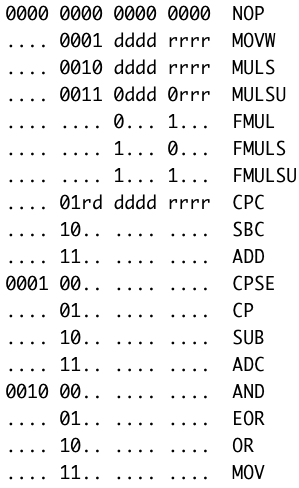
\includegraphics[scale=0.36]{screen1.png}
\end{figure}
\begin{figure}
	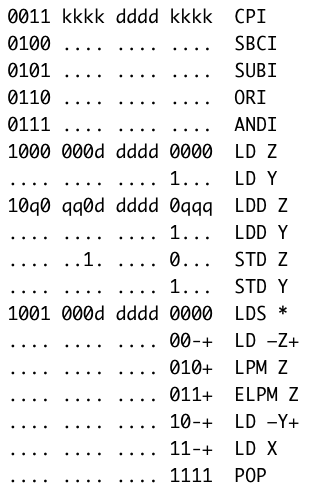
\includegraphics[scale=0.36]{screen2.png}
\end{figure}
\end{multicols}
\end{frame}

\begin{frame}
\frametitle{Patterns II}
\begin{multicols}{2}
\begin{figure}
	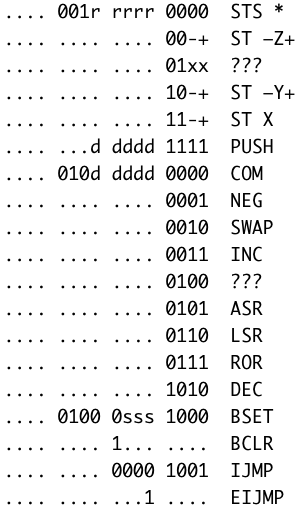
\includegraphics[scale=0.36]{screen3.png}
\end{figure}
\begin{figure}
	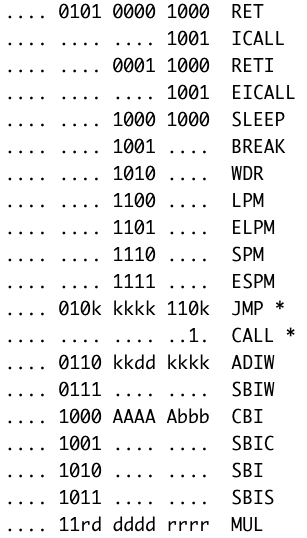
\includegraphics[scale=0.36]{screen4.png}
\end{figure}
\end{multicols}
\end{frame}

\begin{frame}
\frametitle{Patterns III}
\begin{figure}
	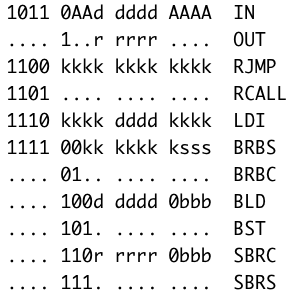
\includegraphics[scale=0.43]{screen5.png}
\end{figure}
\end{frame}

%--------------------------------------------------------

%--------------------------------------------------------
\section{Code Implementation}
%--------------------------------------------------------
\begin{frame}[fragile]
\frametitle{ Macros for help }
\begin{example}[ Macros for bits manipulation ]
\begin{lstlisting}
#define get4Bits(w,B) (((w)&((0xF)<<(B*4)))>>(B*4))
#define getByte(w,B) (((w)&((0xFF)<<(B*8)))>>(B*8))
#define getBit(w,b) (((w)&((0x1)<<b))>>b)
#define shiftBits(w,b) ((w)<<b)
\end{lstlisting}
\end{example}
\begin{example}[ Macros for string processing ]
\begin{lstlisting}
#define clean(s) sprintf((s),"")
#define cut(s,i,sz) ((s).substr((i),(sz)))
#define to_c(s) ((s).c_str())
#define getHex(s,n) (sscanf(s,"%x",&(n)))
\end{lstlisting}
\end{example}
\end{frame}
%--------------------------------------------------------
%--------------------------------------------------------
\begin{frame}[fragile]
\frametitle{ Main function }
\begin{example}[ From .HEX to the world  ]
\begin{lstlisting}
int main() {
   string hexLine, parsedCmd;
   ifstream hexFile;
   int err = 0;	
   //For test purposes
   hexFile.open("main.hex");	
   // Read each line from .hex file while possible
   while (getline(hexFile, hexLine)) {
      // Now parse the string to a more friendly format
      err = parse_cmd(hexLine, parsedCmd);
      if(err)  {
         printf("Error ocurred %d\n",err);
         break; 
      }
      // If no errors proceed to execute the command	
      split_cmds(parsedCmd);
   }
   return 0;	
}
\end{lstlisting}
\end{example}
\end{frame}
%--------------------------------------------------------
%--------------------------------------------------------
\begin{frame}[fragile]
\frametitle{ Parsing .HEX file }
\begin{example}[ More detailed in code]
\begin{lstlisting}
int parse_cmd(string &str, string &cmds) {
   int byteCount, address, recordType, checkSum, idx = 1;
   . . .
   /* Byte Count: */
   getHex(to_c(cut(str,idx,2)),byteCount);
   idx += 2;
   /* Address: four hex digits */
   getHex(to_c(cut(str,idx,4)),address);
   idx += 4;
   /* Record type: two hex digits */
   getHex(to_c(cut(str,idx,2)),recordType);
   idx += 2;
   /* Data: n bytes of data */
   cmds = cut(str,idx,2*byteCount);
   idx += 2*byteCount;
   /* Checksum, two hex digits */
   getHex(to_c(cut(str,idx,2)),checkSum);
   return checksum_ok(str, idx, checkSum);
}
\end{lstlisting}
\end{example}
\end{frame}
%--------------------------------------------------------
%--------------------------------------------------------
\begin{frame}[fragile]
\frametitle{ Return true when the checksum of hex line is OK }
\begin{example}[ C++ Implementation ]
\begin{lstlisting}
int checksum_ok(string &str, int &size, int &checkSum) {
   unsigned int check=0;
   int twoByte, i=1;
   for(; i< size; i += 2) {
      getHex(to_c(cut(str,i,2)),twoByte);
      check += twoByte;
      check &= 0xFF;
   }
   // Two complement of a function
   check = (~check) + 1;
   check &= 0xFF;
   // Verify against checksum expected
   return (check != checkSum) ? -EINVAL : 0;
}
\end{lstlisting}
\end{example}
\end{frame}
%--------------------------------------------------------
%--------------------------------------------------------
\begin{frame}[fragile]
\frametitle{ Split Commands  }
\begin{example}[ Also verify endianess  ]
\begin{lstlisting}
void split_cmds(string &cmds) {
   // We had blocks of 4 bytes, lets process them
   int opCode, swapCode;
   for(int i=0; i<cmds.size(); i += 4) {
      getHex(to_c(cut(cmds,i,4)),opCode);
      /** Now that we know each opcode lets 'execute' them
      * Each opcode is an int of 16 bits
      **/
      if(little_endian) {
         /* We have to swap the byte order to Endianess */
         swapCode  = shiftBits(getByte(opCode,0),8);
         swapCode |= shiftBits(getByte(opCode,1),0);
         opCode = swapCode;
      }
      execute_cmd(opCode);
      }
}
\end{lstlisting}
\end{example}
\end{frame}
%--------------------------------------------------------
%--------------------------------------------------------
\begin{frame}[fragile]
\frametitle{ Executing Commands }
\begin{example}[ Each function will handle the OpCode ]
\begin{lstlisting}
// Axzz Array to select based on the first bytes
Handler oAxzz[] = {
    op0xzz,   op1_2xzz, op1_2xzz, op3_7xzz,
    op3_7xzz, op3_7xzz, op3_7xzz, op3_7xzz,
    op8xzz,     op9xzz,   opAxzz,   opBxzz,
    opC_Dxzz, opC_Dxzz,   opExzz,   opFxzz
};

// Choose the right command to execute  
void execute_cmd( int &opCode ) {
   int A = get4Bits(opCode,3);
   // Delegate the responsibility to next functions
   oAxzz[A](opCode);
}
\end{lstlisting}
\end{example}
\end{frame}
%--------------------------------------------------------
%--------------------------------------------------------
\begin{frame}[fragile]
\frametitle{ Example of OpCode decodification}
\begin{example}[When the 2 most significative nibble is within range 3,7]
\begin{lstlisting}
void op3_7xzz(int &opCode){
   int k = shiftBits(get4Bits(opCode,2),8);
        k += get4Bits(opCode,0);
   int A = get4Bits(opCode,3);
   int d = get4Bits(opCode,1);
   string cmd, param;
   string cmds[] = {"cpi","sbci","subi","ori","andi"};
   cmd = cmds[A - 0x3];
   sprintf(tmp,"R%d, %d",d,k);
   param = tmp;
   AVR_EXE("%s\n",to_c(cmd+" "+param));
}
\end{lstlisting}
\end{example}
\end{frame}
%--------------------------------------------------------
%--------------------------------------------------------
\begin{frame}
\frametitle{ References }
\begin{itemize}
	\item http://lyons42.com/AVR/Opcodes/AVRAllOpcodes.html
	\item http://www.avrfreaks.net/forum/looking-avr-opcode-table
	\item https://en.wikipedia.org/wiki/Intel\_HEX
\end{itemize}
\end{frame}

\end{document} 
